\documentclass[twocolumn, letterpaper,13pt]{scrartcl}

\usepackage{uog_factsheet}
\usepackage{xcolor}
\usepackage{hyperref}

\definecolor{seablue}{RGB}{0,127,169}

\begin{document}
    \title{\color{seablue}Analysis of the NHS's personal data handling in the context of GDPR and Brexit}

	\maketitle
	
    \section*{Introduction}
    
        The \textbf{National Health Service}\cite{link} (NHS) is a catch-all term for the publicly-funded healthcare systems of the United Kingdom (UK). System\textit{s} plural as the NHS has four instances deployed across the UK: England, Wales, Scotland, and Northern Ireland.
        
        In view of the political events surrounding Brexit, \textbf{the UK ceased being part of the European Union (EU) on December 31\textsuperscript{st}, 2020}. As such, the current status of NHS' privacy and cookie policies with regards to the General Data Protection Regulation (GDPR) enters a transition phase that is worth studying.

	\section{The NHS and GDPR's application}
	
	    By leaving the EU, the UK has become a "\textbf{Third Country}\footnote{Before that, for GDPR purposes, the NHS’s basis for lawful processing was Article 6(1)(e), ‘exercise of official authority’; Article 9(2)(h), ‘health or social care’; Article 9(2)(i), ‘public health’; Article 9(2)(j), ‘archiving […] research […] or statistical purposes’\cite{nhsengland}.}" as per the statuses of GDPR\cite{thirdCountriesStatus} (e.g. GDPR's \textit{Article 44 on General Principle for Transfers}) and the decisions made by the European Commission\cite{thirdCountryNote}. 
	    
	    The status of "Third Country" means that GDPR will "\textit{restrict the transfer of personal data to the UK unless the data is protected in another way. For example, via a data adequacy agreement, which provides blanket agreement for data to flow from the European Economic Area (EAA) to a specified third country}"\cite{dataAdequacyAndBrexit}. A country with a data adequacy agreement is considered a \textbf{secure third country} (e.g. Israel) compared to other third countries. 
	    
	    \subsection{Brexit and end of the transition period}
	    As of today, \textbf{the UK is not considered a secure third country as no data adequacy agreement has been legislated}, notably on political concerns regarding data-sharing agreements with other non-EU countries\cite{USagreement}. In Consequently, the NHS is impacted by GDPR in a novel and restrictive way and its data officers will have to implement mitigating actions.
	    
	    \subsection{NHS data officers' necessary mitigating actions}
	    
	    Without a data adequacy agreement, the NHS is currently facing the following GDPR hurdles\cite{dataAdequacyAndBrexit} enforced on institutions and companies operating from a "third country":
	    \begin{itemize}
	        \item Further obstacles impacting NHS' reciprocal healthcare arrangements
	        \item Reduced avenues to query and retrieve early warning data from EU-based data-sharing platforms and alert systems
	        \item Potential cut from EU-based data in the context of UK medical research
	        \item Impaired patient care, research, etc. data-flow to and from the EU
	    \end{itemize}
	    
	\section{Website Registration}
	
	    According to the Internet Assigned Numbers Authority (IANA)\cite{iana}, the website affiliated to the NHS is registered in the United Kingdom, cementing the status that the NHS is operating from a third country.
	    
	   \begin{quote}\textit{\% IANA WHOIS server}\newline
        refer:        whois.nic.uk\newline
        domain:       UK\newline
        organisation: Nominet UK\newline
        address:      Minerva House\newline
        address:      Edmund Halley Road\newline
        address:      Oxford Science Park\newline
        address:      Oxford  OX4 4DQ\newline
        address:      United Kingdom
        \end{quote}
	    
	\section{The NHS and potential EU-based users}
	
	    Because of its position as a European country, the UK has relatively large population exchanges with continental Europe that it will have users (e.g. UK citizens) located in the EU, either temporarily or permanently\footnote{As of 2018, 784,900 British citizens lived in the EU\cite{euBritStats}.}.
	    
	    This taken into account, GDPR's Art. 3 on "Territorial Scope" stipulates that the regulation applies to the processing of personal data within the confines of the EU regardless tooof the origin of the data subject\cite{art3}. Thus, \textbf{the NHS will have to adhere to the GDPR regulation when dealing with its users whenever they are located in the EU}.
	    
	    The way the NHS has dealt with British retirees drawing a UK pension\footnote{This situation led to the UK government creating new administrative processes such as the S1 form to manage financial ('exportable benefits') and data flows to and from the EU.} and British expats entitled to UK-paid healthcare\cite{pensionsAndHealthcare} will have to adapt when they are located in the EU. The data of those NHS users is undoubtedly be covered by GDPR. Furthermore, holders of a European Healtcare Insurance Card\cite{ehic} (for instance for "au Pair" workers) will also be concerned.
	
	\section{NHS' cookie banner and user interaction with cookies}
	
	    The website front page displays a cookie banner (see Fig. \ref{fig:a}) linking to the NHS' cookie policy\cite{cookiepolicy} (reproduced Annex 1) that further links to others such as its privacy policy\cite{privacypolicy} (reproduced in Annex 2). 
	    
	    \begin{figure}	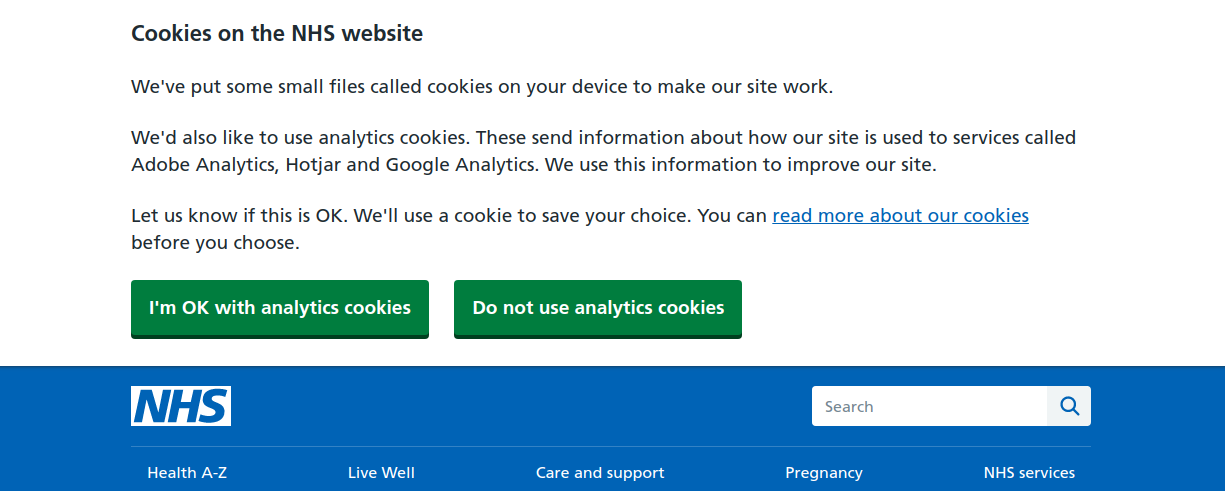
\includegraphics[width=0.98\linewidth]{nhs_cookie_bar.png}
     		\caption{NHS Cookie Banner\label{fig:a}}
      	\end{figure}
	
	To comply with the GDPR's cookie rules, the NHS' website and its data controller must\cite{cookieGDPR}:
    \begin{itemize}
        \item Request and receive users’ consent before any use of cookies except strictly necessary ones.
        \item Provide accurate and specific information about the data being tracked and the purpose in plain language.
        \item Document and store users' consent.
        \item Allow users to access the NHS' service even in case of a refusal.
        \item Make it as easy for users to withdraw/change their consent choices.
    \end{itemize}
	
	\subsection*{NHS' compliance with GDPR with regards to EU-based users}
	
	Based on the assumption that connecting to the website from a EU IP enables the website to adapt its presentation of its cookie policy, we find the following:
	
	\begin{itemize}
	    \item Users are informed via the cookie banner that the site contains cookies "to make [it] work", implying that the website contains mandatory cookies the user cannot opt out of (see Fig. \ref{fig:b}).
	    \item With regards to non-mandatory cookies, called "analytics cookies" by the NHS, the users can opt-out of. Accurate and specific information about the data collected and its purposes is stated. The NHS distinguishes those in three categories (see Fig. \ref{fig:c})
	    \item Cookie consent is documented and stored for 1 year (See Fig. \ref{fig:b} at "CookieConsent"). 
	    \item NHS' services are not impacted by opting out of cookies\cite{cookiepolicy}. The NHS states: "some cookies, like those used to measure how you use our website, are not needed for our website to work."
	    \item Changing one's consent is easily done via a specific and exhaustive cookie setting page\cite{cookiesettings}.
	\end{itemize}
	
	\subsection*{User interactions with cookies}
	
	There are three layers related to cookies that data subjects can interact with:
	
	\begin{itemize}
	    \item cookie consent bar
	    \item cookie policy page (accessible from the bar)
	    \item cookie setting page (accessible from the policy)
	\end{itemize}
	
	With regards to consent related to EU-based users, and given the policy\cite{cookiepolicy} and settings\cite{cookiesettings} available as well as the used cookies (See Fig. \ref{fig:b}, Fig. \ref{fig:c}), it can be noted that consent is \textbf{freely given}\footnote{Note in Fig. \ref{fig:a} that there are no distinguishable color features that makes the button accepting the policy more attractive than the other one, hinting that no dark pattern is being used here}. It is also \textbf{specific} (The data subject can refuse analytics cookies from the consent bar, then can proceed to the setting page to personalize their choice without hindrance), \textbf{informed} (each cookie in the policy and setting pages is clearly stated with a description and an expiration date), \textbf{with a provided policy}. Overall cookie use appears \textbf{unambiguous} and without condition/retaliation and with a right to revocation.
	
	As such, \textbf{no glaring issues arises on the ground of cookie consent, usage and reach by the NHS}.

    \begin{figure}	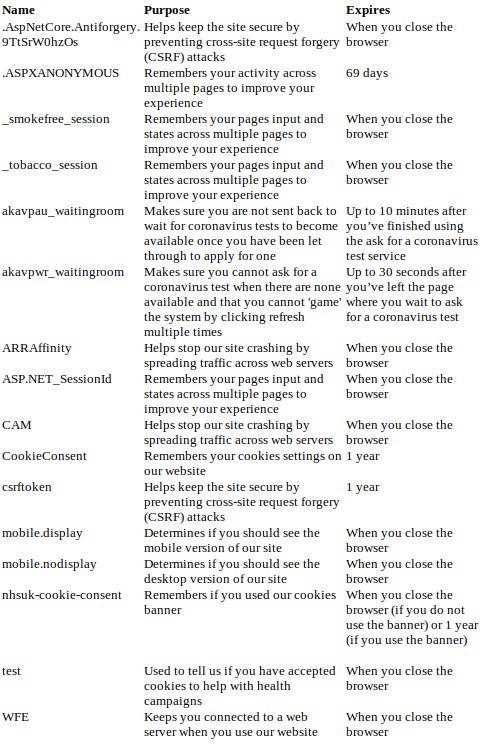
\includegraphics[width=0.98\linewidth]{mandatory_cookies.png}
    \caption{Mandatory Cookies\label{fig:b}}
    \end{figure}

	\section{NHS' privacy and cookie policies}
	
	    The NHS provides an exhaustive and compliant cookie policy that suits its role as an institution providing a public service. The website states clearly their users' rights\cite{gdprfurther} (reproduced in Annex 3) and displays an exhaustive privacy policy as well.
	    
	    \begin{figure}	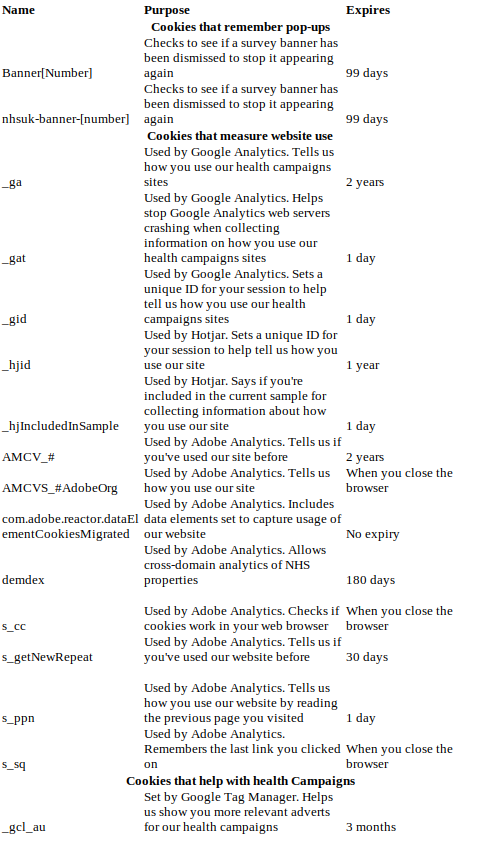
\includegraphics[width=0.98\linewidth]{analytics_cookies.png}
        \caption{Analytics Cookies\label{fig:c}}
        \end{figure}
	    
	    As previously stated, collected data by the NHS fall into the personal data category in specific cases related to users' location. Indeed, let's recall GDPR Art.4's definition of Personal Data, i.e. "\textit{any information relating to an identified or identifiable natural person (‘data subject’); an identifiable natural person is one who can be identified, directly or indirectly, in particular by reference to an identifier such as a name, an identification number, location data, an online identifier or to one or more factors specific to the physical, physiological, genetic, mental, economic, cultural or social identity of that natural person.}" This, along with the territoriality clause of GDPR Art. 3, implies that the data collected by the NHS from people residing or vacationing in the EU will be considered personal data under GDPR.
	    
	    \subsection*{Stated purpose of the data collection}
	    
	    The NHS states that the data it collects with cookies covers the following purposes:
	    
	    \begin{itemize}
	    \item make the website work, for example by keeping it secure
        \item remember which pop-ups the user has seen
        \item measure how the user uses the website, such as which links is clicked on (analytics cookies)
        \item help show the user relevant health campaigns on social media
        \end{itemize}

	    With those purposes and the definitions stated above, we can look deeper into the types of cookies on the NHS' website and see whether or not they aggregate personal data. We focus here on the opt-out analytics cookies (See Fig. \ref{fig:c} and policy\cite{cookiepolicy}), which can be separated into 3 categories: 
	    \begin{itemize}
	    \item Cookies that remember pop-ups -- These cookies remember pop-ups seen and actions done by users. The NHS uses that knowledge to adapt their experience during new visits. Obviously, this impacts users that are identifiable, directly or indirectly. Those choices, when done by British citizens vacationing or living in the EU may be construed as personal data.
        \item Cookies that measure website use (analytics cookies) -- These cookies store information about how users interact with the website. The NHS uses these cookies to help improve the website and more, highlighting two cases with regards to how it relates to personal data:
        \begin{itemize}
            \item the website stores data and makes it identifiable. In this case it’s personal data (e.g. data allowing the NHS to contact British citizens living in the EU).
            \item the website stores data, but makes it anonymous and uses it within a large database of users, e.g., to predict trends. The data loses its personal data type.
        \end{itemize}
        \item Cookies that help with health campaigns: -- These cookies help the website show users relevant ads for the website's health campaigns on social media, such as Facebook or Twitter. In this situation, the consideration of personal data being involved follow a similar route: depending on how it is stored and used, it could be personal data or not (for instance when it involves British people residing in the EU).
        \end{itemize}
        
        Further information on how the data is processed is readily accessible in four available pages covering i) how the NHS looks after users' health and care information\cite{healthandcare}, ii) transparency\cite{transparency}, iii) data and cyber security\cite{cybersec}, iv) and GDPR\cite{gdprfurther}.
        
        \subsection*{The position of the data controller and third-party processors}
        
        As a reminder, a data controller is a company/entity with whom the data subject interacts with. In this case the data controller is the Health and Social Care Information Centre, known as NHS Digital. The information is available in the privacy policy\cite{privacypolicy} (reproduced in Annex 2). Furthermore, the NHS' website mentions a data protection officer (named Kevin Willis) and a Governance Compliance Team (reproduced in Annex 2).

        The NHS controls some dependent services considered data processors\cite{processors} (e.g. NHS' Processing Services, NHS Improvement) from which depend other smaller processors or partners (e.g. Health Data Research UK).

        It is stated that some data are collected on behalf of the NHS by third-party companies whenever a data subject turns on analytics cookies.

        \begin{itemize}
        \item Adobe Analytics, Google Analytics, Hotjar collect data subject's information about how they use the website so as to help improve on it (see third-party section in the privacy policy\cite{privacypolicy})
        \item Hotjar and Qualtrics offer the NHS a suite of survey tools which collects, potentially, personal data on behalf of the NHS (see third-party section in the privacy policy\cite{privacypolicy})
        \end{itemize}
        
        Furthermore, the website video content are streamed to users by a third-party company, Brightcove.
        
        \subsection*{Legal Basis}
        
        The privacy policy clearly states the legal bases of their use of personal data. For instance, it is stated that: "\textit{if we are using your data because we have a legal basis to do so under the Health and Social Care Act, and you do not agree, you have the right to object}" and "\textit{NHS Digital operates the NHS website as directed by the Electronic Prescription Service, Health and Social Care Network, N3, NHS e-Referral Service, Secondary Use Service (SUS), Spine 2 (Named Programmes) Directions 2016 under the powers of sections 254(1) and (6), 274(2), 304(9) and (10) of the Health and Social Care Act 2012. This direction supplements the Health and Social Care Information Centre (Systems Delivery Functions for the NHS website and Additional Systems Delivery Functions for the NHS website) Directions 2013.}"
        
        Beyond those prerogatives and the roles stipulated in the Data Protection Act of 2018, and the cases where GDPR applies (such as with British people living in the EU), a series of 52 directives\cite{directives} which shape the legal basis on which the NHS can operate their data collection via cookies are available to read.
        
    \section{Further Exploration of the Use of Third-Parties on the NHS' website}
	
	    Beyond mentioning the use of third-party cookies in their consent bar (see Fig \ref{fig:a}), the NHS states that five third-party services are used on the website (some of which have already been mentioned in the previous section):
	    \begin{itemize}
        \item New Relic
        \item Adobe Analytics
        \item Google Analytics
        \item Hotjar
        \item Qualtrics
        \end{itemize}
        
        Among those, the cookie setting page\cite{cookiesettings} mentions that Adobe Analytics, Google Analytics, and Hotjar are used to provide cookies to the users. The purpose is clearly stated and the legal basis for each of them is covered (as seen in the \textit{Legal Basis} part of the previous section).
        
        Other third-parties are used on the website to provides services but not cookies (e.g. Bing, CloudFlare (via their CDN), LivePerson, and Vimeo).
        
        The third-parties involving cookies are clearly stated in the privacy policy (reproduced in Annex 2 and see excerpt in Fig. \ref{fig:d}). Furthermore, the privacy policy of each of the five third-parties listed above are provided to the user via hyperlinks.

	\begin{figure} 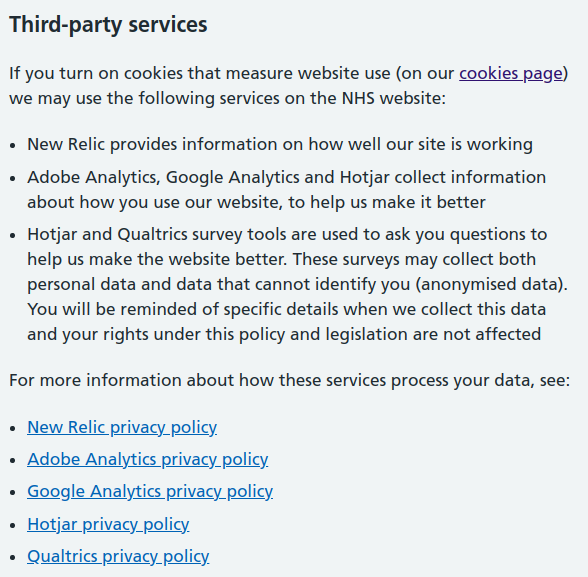
\includegraphics[width=0.98\linewidth]{third_parties.png}
    \caption{Third-party services section\label{fig:d}}
    \end{figure}
    
    Another service, that of comments and ratings moderation is performed by a third-party called ICUC. A point of note here is that the NHS provides a link to the ICUC privacy policy as with the five third-parties above, however this link references the NHS' privacy policy page instead -- a glaring issue.
    
    \subsection*{Using Developer Tools to find non-accounted third-parties}
    
    The developer tools provided by the Chrome browser (See Fig. \ref{fig:e}) help analyze scripts and cookies on a website, to detect present third-parties and related scripts responsible for storing cookie information on a website. 
    
    Our analysis shows that the only third-party scripts loaded on the website are from Adobe Analytics and Hotjar. Interestingly enough, we could not find hints of Google Analytics scripts, though they are mentioned in the privacy policy, cookie policy, and cookie banner. The same goes for Google Analytics cookies.
    
    A research on the Adobe Analytics and Hotjar websites shows that both services are responsible for collecting information on user behaviours during browsing, which matches with what is mentioned in the NHS privacy policy.
    
    The information produced by these cookie scripts indicates that no other third-parties are present on the website. This indicates that the NHS is exhaustive in the list of cookies listed in its policies. While services such as Google Analytics or Adobe Analytics are third-party processors, Most analytics cookies, such as Google Analytics and Adobe Analytics are stored as first-party analytics cookies\cite{google}.
    
	\section*{Conclusion/Overview}
	
	   Overall, we conclude that the NHS likely complies with the current GDPR rules with regards to data subjects covered by the regulation. The previous implementation of GDPR by the website while the UK was part of the EU helps towards this goal.
	   
	   However, the new status of the UK as a third country since January 1st, 2021, and the lack of a data adequacy agreement with the EU implies a certain amount of uncertainty with regards to data transfers to and from the EU. Still, given the current GDPR rules and previous implementation of GDPR by the NHS, the UK's Data Protection Act of 2018, and other directives in place, we are fairly confident in the good implementation and application of GDPR in the future despite this temporary uncertainty.
	
	\begin{figure}	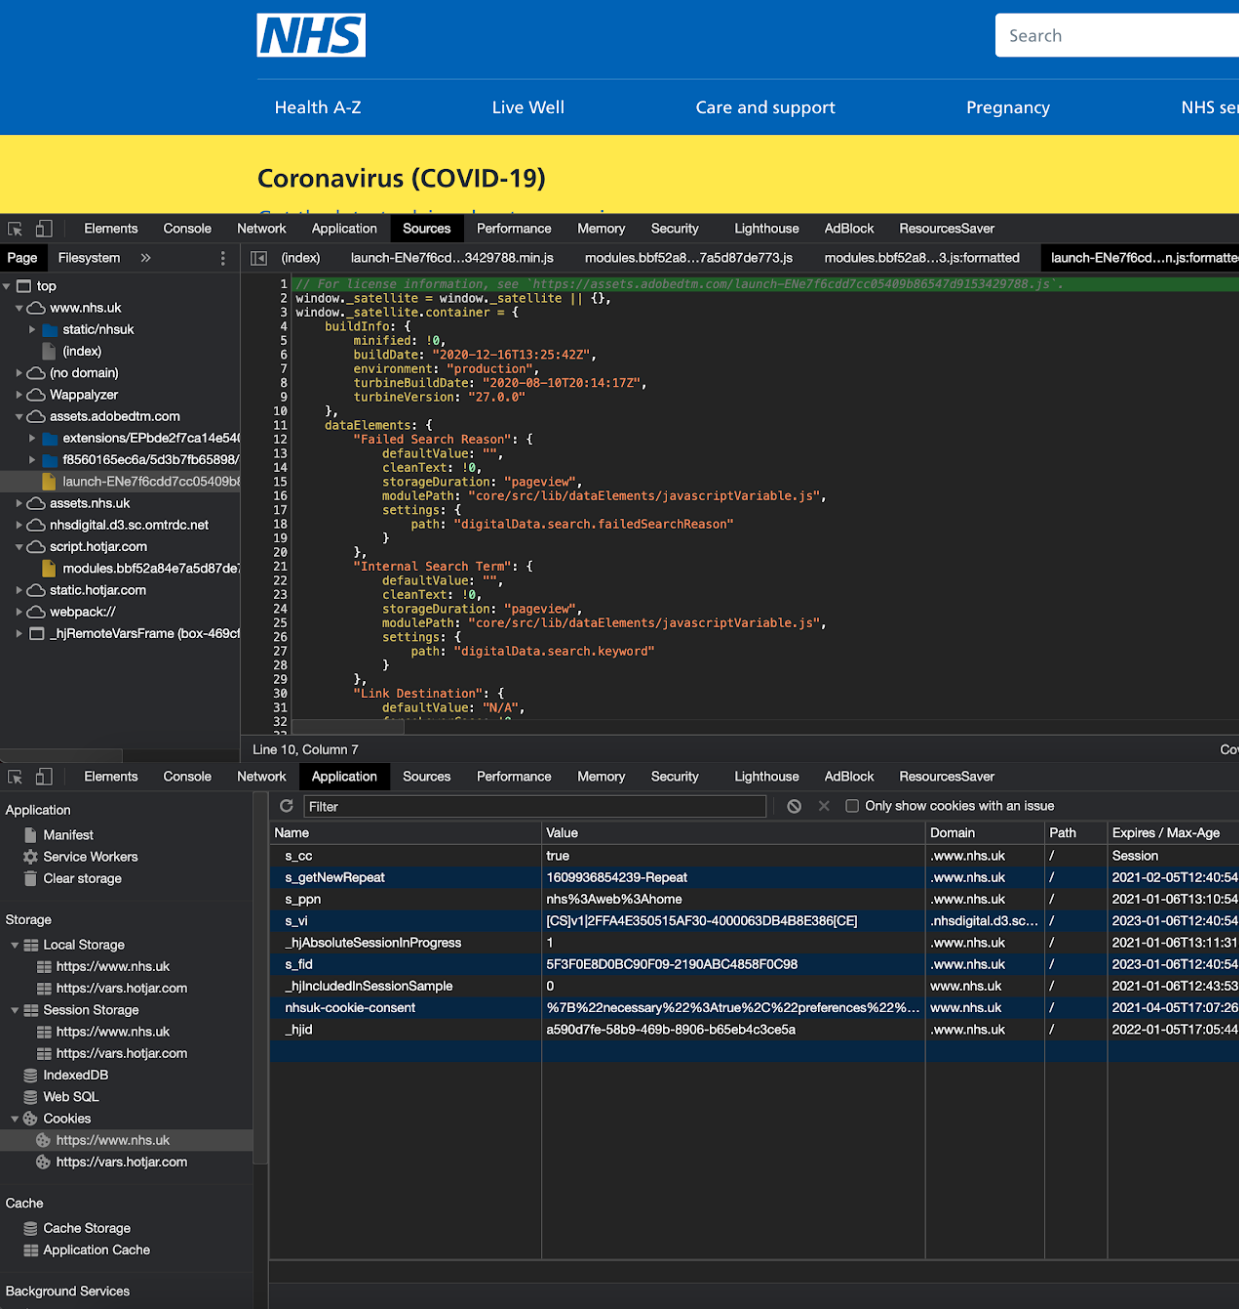
\includegraphics[width=0.98\linewidth]{devtools.png}
    \caption{Chrome Developer Tools to detect third-parties\label{fig:e}}
    \end{figure}
	
	\section*{Annex}

	\subsection*{Annex 1 - Cookie Policy}
	
	\begin{quote}
        \textbf{\textsc{Cookies on the NHS website}}
        
        \textsc{What are cookies?}
        
        Cookies are files saved on your phone, tablet or computer when you visit a website.
        
        They store information about how you use the website, such as the pages you visit.
        
        Cookies are not viruses or computer programs. They are very small so do not take up much space.
        
        \textsc{How we use cookies}
        
        We use cookies to:
        
        \begin{itemize}
            \item make our website work, for example by keeping it secure
            \item remember which pop-ups you've seen
            \item measure how you use our website, such as which links you click on (analytics cookies)
            \item help show you relevant health campaigns on social media
        \end{itemize}
        
        \textsc{Change your cookie settings}
        
        Some cookies, like those used to measure how you use our website, are not needed for our website to work.
        
        These cookies can help us make our website better, but we'll only use them if you say it's OK.
        
        \textsc{How we use the information we collect}
        
        To find out how we collect, store and use information about you or your visit, see the NHS website privacy policy.
        
        \textit{Page last reviewed: 1 April 2019}
        
        \textit{Next review due: 1 April 2022}
	\end{quote}
	
	\subsection*{Annex 2 - Privacy Policy}
	
	\begin{quote}
        \textbf{\textsc{Your privacy on the NHS website}}
        
        \textbf{Our privacy policy}
        
        Your privacy is important to us. This privacy policy covers what we collect and how we use, disclose, transfer and store your information.
        
        \textsc{What information do we collect when you use the NHS website?}
        
        When you use the NHS website, we use various technologies to collect information automatically – such as your IP address. This is commonplace across all internet services to enable the investigation of issues such as service availability and the identification of malicious use. This information is then kept in our internet access logs.
        
        We also collect some personal information directly – for example, when you actively submit details like your postcode to find nearby services.
        
        \textsc{How do we use the information we collect about you?}
        
        We analyse information to see what is most effective about our website and associated services to help us identify ways to improve it and to make it more effective. We may also use information for other purposes, which we would describe to you at the point when we collect the information.
        
        \textsc{Cookies}
        
        Our website uses cookies. These are small files saved on your phone, tablet or computer when you visit a website. They store information about how you use the website, such as the pages you visit.
        
        The law states that we can store cookies on your device if they are strictly necessary for the operation of this site. For all other types of cookies we need your permission before we can use them on your device.
        
        You can:
        
        \begin{itemize}
            \item choose which cookies we use
            \item see details about the cookies we use
        \end{itemize}
        
        \textsc{Video content}
        
        The NHS website video content – whether viewed on the website, in emails or embedded in third-party sites – are streamed to users by a third-party company, Brightcove.
        
        See the Brightcove privacy policy for more information about how they collect and use data about viewers of our videos.
        
        \textsc{Email subscriptions}
        
        If you sign up for one of our email subscription services, we will hold the information you submitted (such as your email address) for as long as we are providing you services.
        
        If you do not access the services provided by us, for instance you do not open or click through one of the emails for more than a year, we will send you an email asking you to confirm that you wish to continue receiving our emails. If you do not respond to this email within 1 month we will unsubscribe you.
        
        We will remove all personal information we hold relating to you, which you registered with us, within 6 months of you unsubscribing from the site. We hold this information for a further 6 months following unsubscription, as we may need to use it for statistical analysis or if you choose to resubscribe. Be assured that if you unsubscribe you will not receive further information from us.
        
        \textsc{NHS website enquiries}
        
        If you contact the NHS website with an enquiry, such as a question about our content, you may be contacted to provide feedback on how we managed your enquiry. You will be asked for your consent when you submit your data to us.
        
        We will hold the information you provide us for as long as necessary to support the service we are providing you, for example so we can continue to provide assistance or resolve an ongoing issue.
        
        If no communication has been made in over 12 months and the information is not required to resolve an ongoing issue, then all communication and any personal information will be deleted. Non-personal information, such as how long your enquiry was open for or the part of the website you were using, will remain. This is to allow for reporting over a period greater than 12 months.
        
        Information is kept for 12 months to allow for trend analysis, identifying reoccurring issues and understanding common issues.
        
        Exceptions include those currently following the complaints process, or when consent to keep information for longer has been obtained. Additionally, if we have determined that the information supplied contains personal information that we do not need to hold to provide assistance, we will endeavour to remove this information sooner.
        
        \textsc{Our interactive tools}
        
        We produce several interactive tools that can help you learn more about your health. For example, our Heart Age tool can help you find out how healthy your heart is.
        
        As well as appearing on the NHS website, these tools can be used on other (third-party) sites.
        
        If you turn on cookies that measure website use (on our cookies page), use of our tools on third-party sites will be tracked. No personal data is collected by these tools.
        
        Information gathered by us includes your IP address, the page a tool is used on, and how many times it is used. In some cases, tracking is used to show user progress through a tool. This information will not be shared with third-parties. All our tools store the number of times a user has visited the tool. Some tools also store information about how far you got through a tool, so you do not have to restart the tool if you use it again.
        
        Some tools, such as the Heart Age tool, allow input of date of birth or postcode, which are converted to age and deprivation score.
        
        \textsc{Third-party services}
        
        If you turn on cookies that measure website use (on our cookies page) we may use the following services on the NHS website:
        
        \begin{itemize}
            \item New Relic provides information on how well our site is working
            \item Adobe Analytics, Google Analytics and Hotjar collect information about how you use our website, to help us make it better
            \item Hotjar and Qualtrics survey tools are used to ask you questions to help us make the website better. These surveys may collect both personal data and data that cannot identify you (anonymised data). You will be reminded of specific details when we collect this data and your rights under this policy and legislation are not affected
        \end{itemize}
        
        For more information about how these services process your data, see:
        
        \begin{itemize}
            \item New Relic privacy policy
            \item Adobe Analytics privacy policy
            \item Google Analytics privacy policy
            \item Hotjar privacy policy
            \item Qualtrics privacy policy
        \end{itemize}
        
        \textsc{Syndication}
        
        We offer a free syndication service that enables partner organisations to pull content from the NHS website via an application programming interface (API) and display it on their website, app or service.
        
        In line with the syndication standard licence agreement, we require personal information of those using this service for contractual purposes. We use the data to inform subscribers of changes to functionality, structure or features within the syndicated content, or if there is a breach of the agreement. We also use subscriber's personal data to feed into internal reports, which identify active callers of the API alongside their usage.
        
        While an active subscriber is receiving syndicated content we will continue to store their personal data. A partner can remove their own account without admin assistance via the API developer portal. Once an account has been closed by either the user or an admin, we will no longer store their data.
        
        \textsc{Service finders}
        
        The website provides a number of service finders to assist you in finding health services near you. While we do not capture any specific information about you as part of this service, the searches, including postcode and other personal information, are saved in our logs and analytics tools. Ideally we would only use part postcodes but this renders the searches ineffectual in rural areas.
        
        \textsc{Comments and ratings}
        
        User comments and ratings are moderated by a service called ICUC. They will receive details of your comment and the name and email address you submit.
        
        See the ICUC privacy policy to find out how they process your information.
        
        We also syndicate published comments and ratings to partner websites, apps or services that adhere to the syndication standard licence terms. We do not pass your email address to our syndication partners.
        
        \textsc{General data services}
        
        We process and publish data in directories on NHS.UK from data aggregators and professional bodies – for example, the British Association for Counselling and Psychotherapy (BACP). This is to provide information to the public about health-related services.
        
        \textsc{Profile Information Management System (PIMS)}
        
        PIMS is used by staff working within dental practices, general practices, pharmacies, opticians, NHS Trusts and social care providers to enter service information on the NHS website so that it can be displayed on the website and syndicated to third-parties.
        
        If you are a PIMS profile editor, we collect personal data from you on registration. The personal data that we collect includes your name, email address, organisation name and job title. We use your personal data to provide the PIMS service and to communicate with you by email for PIMS service related purposes. Occasionally we may contact you for research purposes with the objective of improving the PIMS service or the service information that we provide on the NHS website.
        
        PIMS enables you to add staff information on to your service profile(s). Before doing so, you need to ensure that you acquire and record their consent unless the information is already in the public domain (for example, published on your corporate website or included in a professional body medical register).
        
        \textsc{Social media}
        
        We utilise the following social media platforms to interact with our users:
        
        \begin{itemize}
            \item Facebook (incorporating Instagram)
            \item Twitter
            \item YouTube
        \end{itemize}
        
        \textsc{How the NHS website collects and stores your data}
        
        If you choose to interact with us on social media, we may receive some personally identifiable data about you, which is supplied by the channel you are using (for example, Facebook, Twitter or YouTube). This may include:
        
        \begin{itemize}
            \item name
            \item social media handles (such as Twitter account name)
            \item location history (where you are contacting us from)
            \item images (such as your profile picture)
        \end{itemize}
        
        We will process and store your data in accordance with the terms and conditions and privacy policy of the platform in question. You should be aware that your use of these platforms is governed by the terms and conditions agreed between you and the platform, rather than the NHS website.
        
        We may use social media management tools (such as Hootsuite) to help deliver elements of our service to you. Any personally identifiable data processed using these tools is supplied by the platforms we use, in accordance with their terms and conditions.
        
        We will not remove, duplicate or transfer your personal data from or between any of the social platforms that we use, except for when you give us explicit permission to do so or when we believe that we need to in order to respond to an urgent risk to health.
        
        For example, if you interact with us in a way that raises serious concerns about your mental health, we may share your personal details with local NHS services to ensure that you are offered appropriate support.
        
        You should be aware that social networks may control some of the data associated with interactions between you (the user) and us (the NHS website) on their platforms. For example, we will be able to delete our own records of a private message conversation if you request us to do so, but social networks may store a copy of this conversation that we are unable to access.
        
        We would recommend using the privacy tools built in to the social networks in question to ensure you are able to exercise your rights appropriately.
        
        \textsc{Understanding how social networks use your data}
        
        Social networks use information about your online activity to build a profile of you. This data is then used (anonymously) to send you targeted adverts across various digital platforms.
        
        You should be aware that interacting with health-related accounts such as ours may help build the profile of you that social networks maintain, and could potentially result in you receiving adverts related to health issues.
        
        This process of collecting data for advertising purposes is not controlled by the NHS website, and we do not have access to the profiling data stored by social networks about you.
        
        \textsc{How long do we hold this information?}
        
        Unless otherwise stated, business information that falls under NHS Digital is held for a minimum of 3 years and will be subject to review. We will hold the information for as long as we are providing you services.
        
        \textsc{Do we share information?}
        
        we strive to capture the minimal amount of personal data, and only share with other organisations where the law permits us to do so or where we require and have gained your consent
        
        we only share information with our authorised Data Processors for the sole purpose of processing the data in connection with the service we have procured from them. These processors must act at all times on our instructions as the Data Controller under the Data Protection legislation
        
        we do not sell individuals' information
        
        we host health information campaigns on behalf of Public Health England, where we are Data Processors. These campaigns may have separate privacy terms and consent requirements
        
        before you submit any information, you will be informed why we are asking for specific information and it is up to you whether you provide it
        
        \textsc{How can you access, amend or withdraw the personal data you have given us?}
        
        To get in touch about these rights, please contact us via the Data Controller details above. We will seek to deal with your request without undue delay, and in any event within 1 month (subject to any extensions to which we are lawfully entitled).
        
        *Please note that we may keep a record of your communications to help us resolve any issues that you raise.
        
        \textsc{Right to object}
        
        if we are using your data because we have a legal basis to do so under the Health and Social Care Act, and you do not agree, you have the right to object. We will respond to your request within the required time frame (although we may be allowed to extend this period in certain cases). Generally, we will only disagree with you if certain limited conditions apply
        
        this right enables you to object to us processing your personal data where we do so for one of the following reasons: (i) to enable us to perform a public task or exercise official authority; (ii) to send you direct marketing communications; and (iii) for research or analytical purposes
        
        \textsc{Right to withdraw consent}
        
        Where we have obtained your consent to process your personal data, or consent to send you information, you may withdraw your consent at any time and we will cease to carry out the particular activity that you previously consented to, unless we consider that there is an alternative reason to justify our continued processing of your data for this purpose, in which case we will inform you of this condition.
        
        \textsc{Data access requests}
        
        You may ask us to confirm what information we hold about you at any time, and request us to modify, update or delete such information. We may ask you to verify your identity and for more information about your request.
        
        If we provide you with access to the information we hold about you, we will not charge you for this. If we refuse your request for any legitimate reason, we will always tell you the reasons for doing so.
        
        \textsc{Right to remove}
        
        In certain situations, you have the right to request us to "remove" your personal data. We will respond to your request within the agreed timeframe (although we may be allowed to extend this period in certain cases) and will only disagree with you if certain limited conditions apply.
        
        If we do agree to your request, we will delete your data but will generally assume that you would prefer us to keep a note of your name on a register of individuals who would prefer not to be contacted. That way, we will minimise the chances of you being contacted in the future where your data is collected in unconnected circumstances. If you would prefer us not to do this, you are free to say so.
        
        Normally, the information must meet one of the following criteria:
        \begin{itemize}
            \item the data is no longer necessary for the purpose for which we originally collected and/or processed it
            \item where previously given, you have withdrawn your consent to us processing your data, and there is no other valid reason for us to continue processing
            \item the data has been processed unlawfully (i.e. in a manner that does not comply with existing Data Protection regulations)
            \item it is necessary for the data to be deleted for us to comply with our legal obligations as a data controller
        \end{itemize}
        
        We would only be entitled to refuse to comply with your request for one of the following reasons:
        
        \begin{itemize}
            \item to exercise the right of freedom of expression and information
            \item to comply with legal obligations or for the performance of a public interest task or exercise of official authority
            \item for public health reasons in the public interest
            \item for archival, research or statistical purposes
            \item to exercise or defend a legal claim. When complying with a valid request for the removal of data, we will take all reasonably practicable steps to delete the relevant data
        \end{itemize}
        
        \textsc{Right to restrict processing}
        
        You have the right to request that we restrict our processing of your personal data in certain circumstances.
        
        This means that we can only continue to store your data and will not be able to carry out any further processing activities with it until either: (i) one of the circumstances listed below is resolved; (ii) you consent; or (iii) further processing is necessary for either the establishment, exercise or defence of legal claims, the protection of the rights of another individual, or reasons of important public interest.
        
        The circumstances in which you are entitled to request that we restrict the processing of your personal data are:
        
        \begin{itemize}
            \item where you dispute the accuracy of the personal data that we are processing about you. In this case, our processing of your personal data will be restricted for the period during which the accuracy of the data is verified
            \item where you object to our processing of your personal data for our legitimate interests. Here, you can request that the data be restricted while we verify our grounds for processing your personal data
            \item where our processing of your data is unlawful, but you would prefer us to restrict our processing of it rather than erasing it
            \item where we have no further need to process your personal data but you require the data to establish, exercise or defend legal claims
        \end{itemize}
        If we have shared your personal data with third-parties, we will notify them about the restricted processing unless this is impossible or involves disproportionate effort. We will, of course, notify you before lifting any restriction on processing your personal data.
        
        \textsc{Right to rectification}
        
        You also have the right to request that we rectify any inaccurate or incomplete personal data that we hold about you. If we have shared this personal data with third-parties, we will notify them about the rectification unless this is impossible or involves disproportionate effort.
        
        Where appropriate, we will also tell you which third-parties we have disclosed the inaccurate or incomplete personal data to. Where we think that it is reasonable for us not to comply with your request, we will explain our reasons for this decision.
        
        \textsc{Purpose and legal basis for processing}
        
        NHS Digital operates the NHS website as directed by the Electronic Prescription Service, Health and Social Care Network, N3, NHS e-Referral Service, Secondary Use Service (SUS), Spine 2 (Named Programmes) Directions 2016 under the powers of sections 254(1) and (6), 274(2), 304(9) and (10) of the Health and Social Care Act 2012.
        
        This direction supplements the Health and Social Care Information Centre (Systems Delivery Functions for the NHS website and Additional Systems Delivery Functions for the NHS website) Directions 2013.
        
        \textsc{Keeping information secure}
        
        We invest significant resources to protect your personal information, from loss, misuse, unauthorised access, modification or disclosure. However, no internet-based site can be 100\% secure and so we cannot be held responsible for unauthorised or unintended access that is beyond our control.
        
        \textsc{The NHS website Data Controller}
        
        \begin{itemize}
            \item the Health and Social Care Information Centre (known as NHS Digital) is the Data Controller for the NHS website
            \item the Data Protection Officer is Kevin Willis
            \item find out how NHS Digital looks after your health and care information
            \item if there are any queries regarding this privacy policy, you may contact us using the information below:
        \end{itemize}
        
        Information Governance Compliance Team
        NHS Digital
        1 Trevelyan Square
        Boar Lane
        Leeds LS1 6AE
        
        or email enquiries@nhsdigital.nhs.uk
        
        \begin{itemize}
            \item in some cases, the NHS website is acting as a Data Processor on behalf of another Data Controller e.g. Health Campaigns by Public Health England
            \item we will process your data in accordance with the Data Protection regulations in force in the UK at the time
            \item you are entitled to know whether we hold information about you and, if we do, to have access to that information and require it to be corrected if it is inaccurate
            \item you also have the right to lodge a complaint with the Information Commissioner's Office. Contact the ICO
        \end{itemize}
        
        \textit{Page last reviewed: 12 November 2018}
        
        \textit{Next review due: 12 November 2021}
	\end{quote}

    \subsection*{Annex 3 - Your Rights}
    \begin{quote}
        Data protection laws in the UK give people a number of rights concerning their personal data. Not all rights apply equally to all our processing activity as certain rights are not available depending on the lawful basis for the processing.
        
        When you view an entry in our register of processing activities, we have highlighted which rights apply and which may not. To help understand why some may not apply the following should help.
        
        Examples of where rights may not apply - where our lawful basis is:
        
        Public Interest (Task) then rights of erasure, portability do not apply.
        Legal Obligation then rights of erasure, portability, objection, automated decision making and profiling do not apply
        If you require further detail each link below will take you to the Information Commissioner’s Office’s website where further detail is provided in section ‘When does the right apply’.
        
        These rights are:
        \begin{itemize}
            \item Right to be informed
            \item Right of access
            \item Right to rectification
            \item Right to erasure
            \item Right to restrict processing
            \item Right to data portability
            \item Right to object
            \item Rights in relation to automated decision making and profiling.
        \end{itemize}
        
        We want you to feel confident that we look after everyone’s personal data in line with the law. If you have any questions about your rights, you can get in touch with us at enquiries@nhsdigital.nhs.uk.
    \end{quote}

    \bibliographystyle{unsrtnat}   
    \begin{thebibliography}{9}

    \bibitem{link}
    	NHS' website front page, \textit{\href{https://www.nhs.uk/}{nhs.uk}}.
    \bibitem{nhsengland}
    	NHS' \textit{\href{https://www.england.nhs.uk/contact-us/privacy-notice/how-we-use-your-information/covid-19-response/nhs-covid-19-data-store/}{legal basis for processing data}} as per GDPR.
    \bibitem{thirdCountriesStatus}
    	GDPR-info's note on Third Countries, \textit{\href{https://gdpr-info.eu/issues/third-countries/}{link} with further sources provided}.
    \bibitem{thirdCountryNote}
    	European Commission's \textit{\href{http://ec.europa.eu/newsroom/just/document.cfm?action=display&doc_id=49245}{Note to Stakeholders on the Withdrawal of the United Kingdom from the Union and EU Rules in the Field of Data Protection}}.
    \bibitem{dataAdequacyAndBrexit}
    	NHS Confederation (body that brings together and speaks on behalf of organisations that plan, commission and provide NHS services in the UK)'s  \textit{\href{https://www.nhsconfed.org/resources/2020/11/data-adequacy-and-brexit}{note on Data Adequacy and Brexit}}.
    \bibitem{USagreement}
    	\textit{\href{https://gdpr.report/news/2020/06/18/post-brexit-uk-adequacy-decision-at-risk-due-to-data-sharing-agreement-with-us/}{Post-Brexit UK adequacy decision at risk due to data-sharing agreement with US}}.
    \bibitem{iana}
    	\textit{\href{https://www.iana.org/whois}{IANA WHOIS Service}}.
    \bibitem{euBritStats}
    	 Office for National Statistics' \textit{\href{https://www.ons.gov.uk/peoplepopulationandcommunity/populationandmigration/internationalmigration/articles/livingabroad/april2018}{British residents report}} from April 2018.
    \bibitem{art3}
    	Art. 3 GDPR, \textit{\href{https://gdpr-info.eu/art-3-gdpr/}{Territorial Scope}}.
    \bibitem{pensionsAndHealthcare}
    	NHS' \textit{\href{https://www.nhs.uk/using-the-nhs/healthcare-abroad/moving-abroad/planning-your-healthcare/}{healthcare guidance}} on receiving benefits and healthcare abroad.
    \bibitem{ehic}
    	\textit{\href{https://www.nhs.uk/using-the-nhs/healthcare-abroad/apply-for-a-free-ehic-european-health-insurance-card/}{UK EHIC}} continues to be valid in the EU.
    \bibitem{cookiepolicy}
    	NHS'  \textit{\href{https://www.nhs.uk/our-policies/cookies-policy/}{cookie policy}}.
    \bibitem{privacypolicy}
    	NHS'  \textit{\href{https://www.nhs.uk/our-policies/privacy-policy/}{privacy policy}}.
    \bibitem{processors}
    	NHS'  \textit{\href{https://digital.nhs.uk/data-and-information/data-insights-and-statistics/improving-our-data-processing-services/}{data processing}} activities and partners.	
    \bibitem{cookieGDPR}
    	GDPR's \textit{\href{https://gdpr.eu/cookies/}{mandatory compliance}} with regards to cookies.
    \bibitem{cookiesettings}
    	NHS'
    	\textit{\href{https://www.nhs.uk/our-policies/cookies-policy/cookie-settings/}{cookie setting page}}.
    \bibitem{healthandcare}
    	NHS' \textit{\href{https://digital.nhs.uk/about-nhs-digital/our-work/keeping-patient-data-safe/how-we-look-after-your-health-and-care-information/understanding-the-health-and-care-information-we-collect}{Understanding the health and care information we collect}} page.
    \bibitem{transparency}
    	NHS' \textit{\href{https://digital.nhs.uk/about-nhs-digital/our-work/keeping-patient-data-safe/gdpr/gdpr-register}{Transparency notice: how we use your personal data}} page.
    \bibitem{cybersec}
    	NHS' \textit{\href{https://digital.nhs.uk/cyber-and-data-security}{Cyber and data security}} page.
    \bibitem{gdprfurther}
    	NHS' \textit{\href{https://digital.nhs.uk/about-nhs-digital/our-work/keeping-patient-data-safe/gdpr}{General Data Protection Regulation (GDPR) - information}} page.
    \bibitem{directives}
    	\textit{\href{https://digital.nhs.uk/about-nhs-digital/corporate-information-and-documents/directions-and-data-provision-notices/secretary-of-state-directions}{List of directives}} that the NHS must follow, forming its legal basis of action for data collection via cookies.
    \bibitem{google}
    	Drill-down on \textit{\href{https://www.glideagency.com/blog/2018/04/10/all-you-need-to-know-about-the-google-analytics-cookie}{Google Analytics Cookies}} by Glide Agency.
    
    % \bibitem{aaa}
    % 	aaaaa \textit{\href{aaaa}{aaaa}}.
    	
    \end{thebibliography}

\end{document}